\chapter{Clean Architecture}
\section{Plugins}
\subsection{Datenbank}
Die Datenbank stellt eines der Plugins dar. Als Technologie wurde hier eine SQLite3 Datenbank verwendet. Die konkrete Implementierung der Schnittstelle zur SQLite-Datenbank befindet sich in der Klasse \href{https://github.com/moorts/Morik/blob/main/src/plugins/database/SQLiteDatabase.h}{\textit{SQLiteDatabase}}. Diese Klasse erbt von der abstrakten Klasse \href{https://github.com/moorts/Morik/blob/main/src/adapters/database/AbstractSqlDatabase.h}{\textit{AbstractSqlDatabase}}, die sich in der Adapterschicht befindet. Hierdurch wird eine Dependency Inversion erreicht, da nun eine \textit{AbstractSqlDatabase} von anderen Klassen verwendet werden kann, um SQL-Befehle auf der Datenbank auszuführen, statt eine konkrete \textit{SQLiteDatabase} zu verwenden, was die Abhängigkeit von innen nach außen laufen lassen würde.

\subsection{Verschlüsselung}

Ein weiteres Plugin ist die Verschlüsselungsbibliothek. Als solche wurde Cryptopp\footnote{\url{https://cryptopp.com/}} verwendet. Die abstrakte Klasse \href{https://github.com/moorts/Morik/blob/main/src/application/Cipher.h}{\textit{Cipher}} definiert die Schnittstelle in der Applikationsschicht, die das Plugin implementieren muss. Eine konkrete Implementierung dieser Schnittstelle befindet sich in der Klasse \href{https://github.com/moorts/Morik/blob/main/src/plugins/encryption/CBC\_Cipher.h}{\textit{CBC\_Cipher}}. Dadurch findet auch hier eine Dependency Inversion statt, da \textit{Cipher} verwendet werden kann, um Verschlüsselung zu verwenden, statt eine Dependency auf eine konkrete Klasse der Pluginschicht zu brauchen. Die Schnittstelle muss lediglich einen String ver- und entschlüsseln können unter Angabe des Klar- bzw. Geheimtextes und eines Schlüssels. \textit{CBC\_Cipher} implementiert dies für die Chiffren, die im \href{https://github.com/moorts/Morik/blob/main/src/plugins/encryption/BLOCK.h}{\textit{BLOCK}} enum aufgezählt sind. Momentan handelt es sich dabei um AES und Serpent, neue Chiffren können allerdings leicht hinzugefügt werden, solange sie von Cryptopp unterstützt werden. Diese werden als Block-Chiffren mit Cipher Block Chaining (CBC) als Betriebsmodus verwendet. Um andere Betriebsmodi, oder Nicht-Blockchiffren zu verwenden, müssten weitere Implementierungen des \textit{Cipher} Interfaces hinzugefügt werden. Dies ist ohne Weiteres möglich, solange ein \textit{String} zür Schlüsselherleitung hinreichend ist.

\subsection{User Interface}

Dieses Plugin Implementiert eine Benutzerschnittstelle für das Programm. Eine solche Schnittstelle ermöglicht Interaktion mit dem Password Manager für einen Benutzer, durch Umsetzung der zentralen Schleife. Bei der Schnittstelle handelt es sich um ein \href{https://github.com/moorts/Morik/blob/main/src/plugins/ui/CommandLineInterface.h}{\textit{CommandLineInterface}}, welches das \href{https://github.com/moorts/Morik/blob/main/src/application/AbstractUserInterface.h}{\textit{AbstractUserInterface}} Interface aus der Applikationsschicht implementiert. Auch hier findet folglich eine Dependency-Inversion statt, da das Plugin abhängig vom Interface aus der Applikationsschicht ist.

\subsection{Pseudo-Zufallszahlen-Generator}

Die Implementierung des \href{https://github.com/moorts/Morik/blob/main/src/application/PasswordGenerator.h}{\textit{PasswordGenerator}}s braucht eine Möglichkeit (Pseudo-)Zufallszahlen zu generieren. Das Interface \href{https://github.com/moorts/Morik/blob/main/src/application/PseudoRandomNumberGenerator.h}{\textit{PseudoRandomNumberGenerator}} ist die Schnittstelle in der Applikationsschicht, die definiert wie ein solcher Generator implementiert werden muss. Konkrete Implementierungen werden von Plugins vorgenommen, indem das Interface vom Plugin implementiert wird. In unserem Fall wird dies von der \href{https://github.com/moorts/Morik/blob/main/src/plugins/prng/MersenneTwister.h}{\textit{MersenneTwister}} Klasse übernommen. Durch die invertierte Abhängigkeit, könnte jedoch jederzeit auf eine andere Implementierung umgestellt werden.

\section{Adapter}
\subsection{Datenbank}
Die Klasse \href{https://github.com/moorts/Morik/blob/main/src/adapters/database/DatabaseInterface.h}{\textit{DatabaseInterface}} implementiert die eigentliche Funktionalität in Form der SQL-Anweisungen und führt diese über eine konkrete Implementierung der \textit{AbstractSqlDatabase} in der Datenbank aus. Somit geht keine Funktionalität verloren, wenn das Plugin durch eine andere Datenbanktechnologie ausgetauscht wird. Die Umsetzung der Funktionalität als SQL-Anweisungen bedeutet jedoch, dass ein Austausch des Plugins nur ohne Weiteres möglich ist, wenn die neue Datenbank ebenfalls eine SQL-Datenbank ist. Handelt es sich bei der neuen Datenbank jedoch beispielsweise um eine noSQL-Datenbank, so muss die Funktionalität, also die Abfragen, angepasst werden. Der Klasse \textit{DatabaseInterface} wird im Konstruktor eine \textit{AbstractSqlDatabase} übergeben, was die Dependency Injection umsetzt. Zusätzlich erbt die Klasse \textit{DatabaseInterface} von der abstrakten Klasse \href{https://github.com/moorts/Morik/blob/main/src/application/AbstractDatabaseInterface.h}{\textit{AbstractDatabaseInterface}}, die sich im Kern befindet, sodass die Abhängigkeit vom Adapter auf den Kern zeigt. Dies setzt also die Dependency Inversion um und ermöglicht Klassen im Kern eine Abhängigkeit auf das AbstractDatabaseInterface zu haben statt auf eine konkrete Implementierung dessen.\\
Auf die Benutzung von Prepared Statements wurde innerhalb des Adapters verzichtet, da die Datenbank lokal ist und nur der Benutzer Befehle auf ihr ausführt. Würde die Datenbank über eine öffentliche Schnittstelle angesteuert werden, so wäre dies nicht zu vernachlässigen.

\subsection{User Interface}

Die Klasse \href{https://github.com/moorts/Morik/blob/main/src/adapters/ui/UiDataHelper.h}{\textit{UIDataHelper}} implementiert die Funktionalität, die ein Benutzer zur Verfügung hat. Namentlich handelt es sich dabei um das Anlegen und Bearbeiten von Passwörtern. Diese Klasse ist separat vom entsprechenden Plugin, damit die Funktionalität nicht abhängig ist, von spezifischen Plugins. Neue User Interfaces können also implementiert/hinzugefügt werden, ohne diese Funktionen erneut zu implementieren.

\section{Applikationskern}

Der Kern des Programmes, befindlich im \href{https://github.com/moorts/Morik/tree/main/src/application}{application} Ordner, ist zuständig für die Umsetzung der Domänenkonzepte und enthält zusätzlich Pure Fabrication Klassen (bspw. \href{https://github.com/moorts/Morik/blob/main/src/application/InstanceManager.h}{\textit{InstanceManager}}) und Interfaces, welche von den Plugins implementiert werden (siehe oben). Die Domänenkonzepte sind eng an die gewünschte Funktionalität der Anwendung gebunden. Sie entsprechen den festen Anforderungen an den Passwort Manager, während andere Funktionalitäten, wie konkrete Verschlüsselungsalgorithmen nicht zwingend notwendig/austauschbar sind. Auf dieser Grundlage wurde die Aufteilung in Kern und Plugins/Adapter gewählt. Der Applikationskern hat keine externen Abhängigkeiten, durch konsequente Anwendung der Dependency-Inversion. 

\begin{figure}[ht]
	\centering
	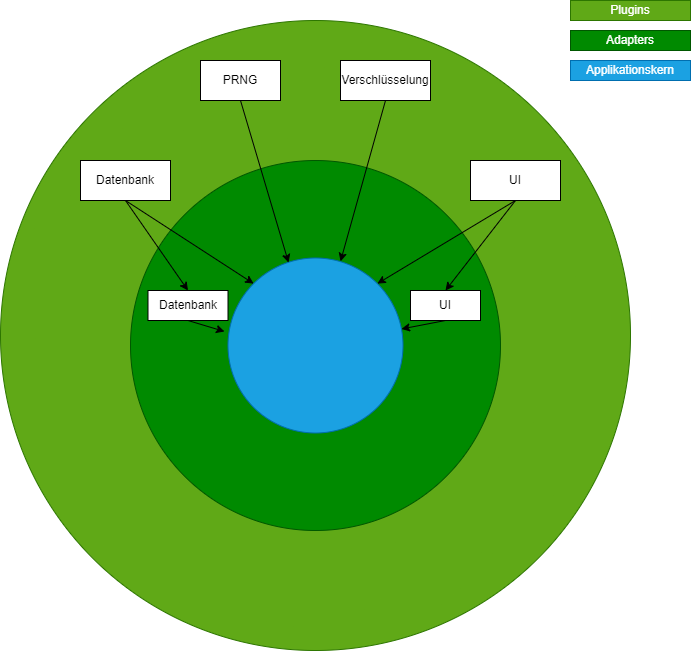
\includegraphics[width=1.0\textwidth]{Bilder/architecture_diagram.png}
	\caption{Abhängigkeitsdiagram}
	\label{fig:CADiag}
\end{figure}

\section{Bewertung}

Die gewählte Architektur war größtenteils angenehm umzusetzen und hat im Endeffekt für ein übersichtliches Projekt gesorgt. Im Laufe der Entwicklung gab es zwar einige fehlerhafte Abhängigkeiten, die korrigiert werden mussten, dies ist jedoch kein Grund für eine Architekturänderung. Neue Funktionen, besonders neue Implementierungen der Interfaces der Applikationsschicht (bspw. der Verschlüsselung), sind einfach umzusetzen.

Alles in allem sind wir zufrieden mit der Architektur und finden sie angemessen für ein Projekt dieser Größe/Form.
